\documentclass[shortpaper]{revdetua}

\usepackage{scicite}
\usepackage{hyperref}

\usepackage{amsmath}
\usepackage{multicol}
\usepackage{setspace}

\usepackage{enumitem}

\usepackage{graphicx}
\usepackage{caption}
\usepackage{float}
\usepackage{subcaption}

\usepackage{verbatim}

\usepackage{booktabs}

%%%%%%%%%%%%%%%%%%%%%%%%%%%%%%%%%%%%%%%%%%%%%%%%%%%%%%%%%%%%%%%%%%%%%%%%%%%%%%%%

\begin{document}
 
\Header{2}{85122}{Dezembro}{2019}{1}

\title{
    \LARGE{{\bf Project 2: Word Counting in Large Texts \/}}
    \vspace{-20pt}
}

\author{
    \Large{{\bf A Study on Exact and Approximate Occurrences Counters\/}}\\\\\\
    Filipe Pires [85122]\\
    \\
    {\bf Advanced Algorithms\/}\\
    \normalsize{Department of Electronics, Telecommunications and Informatics}\\
    \normalsize{University of Aveiro}\\
} 

\maketitle

%%%%%%%%%%%%%%%%%%%%%%%%%%%%%%%%%%%%%%%%%%%%%%%%%%%%%%%%%%%%%%%%%%%%%%%%%%%%%%%%

\begin{abstract}
    The challenge of parallel event counting in a memory efficient way is not
    a recent topic, but it is one still under discussion as there is great room
    for improvement.
    Most of today's solutions perform memory optimization by applying probabilistic 
    counters to estimate the total number of occurrences of events.

    In this report, I focus on two of the most famous approximate counters to 
    determine an estimation of the most used words of literary works from several 
    authors in several languages and compare them to an exact counter.
    I also present a few conclusions drawn from the study applied to the dataset.
\end{abstract}

\begin{keywords}
    Approximate counting, probabilistic counter, memory efficient algorithms 
\end{keywords}

%%%%%%%%%%%%%%%%%%%%%%%%%%%%%%%%%%%%%%%%%%%%%%%%%%%%%%%%%%%%%%%%%%%%%%%%%%%%%%%%

\section{Problem Contextualization}

This report was written for the course of 'Advanced Algorithms', taught by 
professor Joaquim Madeira for the master's in Informatics Engineering at DETI UA.
It describes the work done for the second assignment of the course \cite{trab2}.
The chosen hypothesis was 'C - Approximate Occurrences Counting - Words in Text Files'.

When dealing with large datasets there are many operations that require the 
calculation of properties of each element. 
The presence of data multiple times throughout the data might be a potential
aspect worth exploring.
This is specially true for textual data to determine facts such as how many 
questions exist on a text segment or achieve complex goals like determining 
which language requires less words to convey the same information.
The applicability of solutions to analyse data through occurrence counters is 
wide and most of today's large tech companies know this well.

However, counting events can be very computationally and memory efficiently 
demanding, as for tracking the evolution of independent events (or elements of 
the data) requires a proportional amount of counters constantly updating.
In consequence, there is a great investment in finding improved ways of providing 
such operations through more efficient and scalable algorithms. 
Some of the most famous solutions use counter-based probabilistic algorithms or, 
in particular cases, sketch algorithms (e.g. finding frequent items in data streams).
Examples of probabilistic counters are: counters with fixed or descending 
probabilities; floating-point counters; etc.
What was done for the purpose of the project was to explore the first set of 
approximate counters and compare them to each other and to an exact counter.
With the use of several well known literary works translated into a few languages,
I also describe my observations when comparing languages and mention additional 
relevant conclusions.

%%%%%%%%%%%%%%%%%%%%%%%%%%%%%%%%%%%%%%%%%%%%%%%%%%%%%%%%%%%%%%%%%%%%%%%%%%%%%%%%

\section{Dataset}

To test the performance of the counting techniques, there needed to be prepared 
a sufficiently large dataset for the conclusions to have an actual meaning.
By researching for eBooks from the Gutenberg Project \cite{gutenberg}, I was 
able to build a small collection of 4 literary works translated in 7 languages.
Unfortunately, as the available books were limited, the only common language 
amongst all books was English, although many share other translations.
The configuration is as follows:

\setlist{nolistsep}
\begin{itemize}
    \item \textit{A Christmas Carol}, by Charles Dickens - written in English, Finnish, German, Dutch and French
    \item \textit{King Solomon's Mines}, by H. Rider Haggard - written in English, Finnish and Portuguese
    \item \textit{Oliver Twist}, by Charles Dickens - written in English, French and German
    \item \textit{The Adventures of Tom Sawyer}, by Mark Twain - written in English, Finnish, German and Catalan
\end{itemize}

These books suffered both a manual preprocessing, where I removed the headers and
footers from the files containing details about their source, and an automatic 
filtering during word counting, where punctuation and words considered irrelevant 
for the study are ignored by the counters.
The criteria to decide if a word is relevant is based on a list of stop words 
for all languages of the collection.
These stop words were taken from \cite{nltk} \cite{stopwords}, which basically 
consist of multi language collections of stop words following the ISO standard 
(the first showed better results but the second was the only with stopwords for Catalan).
They contain very common words that lack in useful information about the text under analysis.
During this filtering process, all words with less than 3 letters are also ignored.

%%%%%%%%%%%%%%%%%%%%%%%%%%%%%%%%%%%%%%%%%%%%%%%%%%%%%%%%%%%%%%%%%%%%%%%%%%%%%%%%

\section{Word Counters}

In this chapter I provide a description of how each of the studied counters work,
along with details about their implementations.
The developed code was written in Python, with the help of libraries for word 
counting \cite{lib_counter} through regular expressions \cite{lib_re}, for 
system-related and mathematical operations \cite{lib_sys} \cite{lib_math} and 
random number generation \cite{lib_random}, for graphics generation 
\cite{lib_numpy} \cite{lib_matplotlib} and for file and directory manipulation 
\cite{lib_os} \cite{lib_shutil}.
The file \texttt{WordOccurrenceCounting.py} in the source folder contains 
all functions in a script format.

\subsection{Exact Counter}

The most straightforward counter is the exact counter (henceforward referred to 
as EC). EC's responsibility is to keep track of all words that occur in a text 
given as input and simply increment a counter for each word every time there is 
a new occurrence.
The function \textit{exactCounting()} implements this counter and receives as 
input parameters:

\setlist{nolistsep}
\begin{itemize}
    \item \texttt{books} - a dictionary containing the paths to the books and respective translations to be processed.
    \item \texttt{k} - an integer that defines the number of words to return in descending order of count.
    \item \texttt{study} - an integer that states whether the function is being executed for an elaborate study of not (by default, it is defined for a simple run).
\end{itemize}

EC's implementation stores the results in a global dictionary called 
\texttt{results} and it also calculates additional information such as the total 
number of words counted and the total number of words processed.
Note that the number of processed words will be larger, as many will not be 
considered relevant, as we have seen in the previous chapter.

\subsection{Approximate Counter with Fixed Probability}

The way probabilistic counters work is by incrementing each word's counter if 
a condition is verified. 
This condition involves the random generation of a number and the comparison of
its value with a standard.
In the case of fixed probability counters, the incrementing condition depends 
only on the predefined probability.

For the implementation of the Approximate Counter with Fixed Probability (from 
now on referred to as ACFP), the counter update probability was set to \textbf{0.5},
a value defined \textit{a priori} for the project.
The function \textit{approxCountingFixedProb()} implements ACFP and, when deciding
whether to update the counter of a word or not, it generates a pseudo-random 
integer within the range [1, 100] and checks if it is smaller than the fixed
probability times 100. If so, it proceeds with the increment, else it does not.
A small modification was added to this process to ensure that all words are 
counted at least once by skipping the condition if the Counter object does not 
yet have a counter assigned to the word.
There is an additional parameter passed to \textit{approxCountingFixedProb()} 
besides the ones from EC:

\setlist{nolistsep}
\begin{itemize}
    \item \texttt{prob} - a float value that defines the probability of incrementing the counter.
\end{itemize}

The other 3 parameters, \texttt{books}, \texttt{k} and \texttt{study}, are 
the same for all counter functions, with the exception of \texttt{study} that,
for the approximate counters, its value also defines the identifier of the 
current algorithm run (to distinguish runs in the results).
The idea here is to allow for an elaborate study to be conducted with reduced 
noise, as running a probabilistic algorithm only once is never advisable and does
not usually represent the reality of the algorithm's behavior in general.

\subsection{Approximate Counter \newline with Decreasing Logarithmic Probability}

Finally we have \textit{approxCountingLogarithmic()}, the implementation of the 
ACLP (Approximate Counter with decreasing Logarithmic Probability) that receives
the same parameters as the previous counter except for \texttt{prob} that is 
replaced by:

\setlist{nolistsep}
\begin{itemize}
    \item \texttt{base} - a float value that defines the base for the power that will set the incrementing probability.
\end{itemize}

In this special counter, the incrementing condition depends on the current value 
of the counter itself, meaning that it will be a dynamic condition, unlike ACFP.
The way this works is as follows: when deciding whether to update the counter 
of a word or not, the function generates a pseudo-random integer within the 
range [1, 100] and checks if it is smaller than a calculated probability times 100,
just like ACFP; however, this probability is calculated according to equation \ref{eq:1},
where \texttt{x} is the counter's current value, so as the counter is incremented 
the power grows exponentially and in consequence (since the power is on the 
fraction's bottom portion) the probability decreases logarithmically - hence
the name.
Note that, if there is no counter yet assigned to a given word, the probability 
will be equal to 1, so there is no need to ensure that all words are counted as 
the algorithm already does this by itself.

{\setstretch{0.2}
    \begin{equation} \label{eq:1}
        P(increment) = \frac{1}{base^{x}}
    \end{equation}
}
\vspace{-8pt}

It is important to state that most of the reasoning behind the comprehension and
implementation of these algorithms derives not only from the material of the 
course, but also from Csuros publication on \textit{Approximate Counting with a 
Floating-Point Counter} \cite{csuros} that, although is dedicated to a different 
type of approximate counter, makes an excellent overview of the used counters 
and appropriate performance metrics.

%%%%%%%%%%%%%%%%%%%%%%%%%%%%%%%%%%%%%%%%%%%%%%%%%%%%%%%%%%%%%%%%%%%%%%%%%%%%%%%%

\section{Literary Study}

The main goal of my study was to determine the advantages and disadvantages of 
each approximate counter in a practical way and find out their utility in 
specific contexts.
Notwithstanding, I intended to determine what differences exist in the most 
frequently used words between book translations and, if any, reflect on why they occur.
I also aimed to learn whether any language is capable of conveying the same amount 
of information with fewer words than others - this was not limited to the total 
number of words of course, but also considering the study results.

\subsection{Strategy \& Execution Pipeline}

The study was conducted through the execution of the function 
\textit{elaborateStudy()} that receives as parameters:

\setlist{nolistsep}
\begin{itemize}
    \item \texttt{books} - a dictionary containing the paths to the books and respective translations to be processed.
    \item \texttt{k} - an integer that defines the number of words to return in descending order of count.
    \item \texttt{fixedProb} - a float that defines the probability of incrementing the fixed probability counter.
    \item \texttt{logBase} - a float that defines the base for the power that will set the incrementing probability of the logarithmic counter.
    \item \texttt{n} - an integer that sets the number of times each approximate counter will be executed.
    \item \texttt{out} - a string with the path to the output folder.
\end{itemize}

The values passed to \texttt{books}, \texttt{fixedProb} and \texttt{logBase} 
were already mentioned, and for the remaining parameters I applied the 
configuration \texttt{k=}\textbf{10}, \texttt{n=}\textbf{10} and the outputs were stored in 
the results directory.
The functions execution flow is presented next.

First of all, \textit{exactCounting()} is called once, followed by the execution
of the approximate counters \texttt{n} times.
In this phase all words have an entry on each Counter.

With the \texttt{results} filled, the calculation of the approximate counters'
deviations begins.
All performance metrics are based on the calculation of the deviation between 
the exact count of the number of occurrences of a word and the estimated count 
derived from the counts of the probabilistic solutions.
The way these estimations are calculated differs between Counters, as you may guess.
For the ACFP, this is a straightforward process, requiring only to multiply the 
value on the approximate counter to the fraction $ \frac{1}{fixedProb}$, as seen 
in \ref{eq:2}, that in my case was equal to \textbf{2}, where \textit{E(word)}
refers to the estimated total count of the word.

{\setstretch{0.1}
    \begin{equation} \label{eq:2}
        E(word) = count \times \frac{1}{fixedProb}
    \end{equation}
}

For the ACLP, the deviation was calculated in two distinct ways.
The first way also uses the estimated total count derived from the approximate
counts, following equation \ref{eq:3}.
The second way is the inverse process, where instead of estimating the total count
and comparing it with the true count, the values from EC suffer the transformation
presented in equation \ref{eq:4}, where \textit{LogCount(word)} refers to the 
logarithm of the word's exact count plus 1. This transformation is then compared 
to the values of ACLP's counts.

\begin{equation} \label{eq:3}
    E(word) = \frac{logBase^{count} - logBase + 1}{logBase - 1}
\end{equation}

{\setstretch{0.1}
    \begin{equation} \label{eq:4}
        LogCount(word) = \log_{logBase}{(exactCount+1)}
    \end{equation}
}

All deviations correspond to the distance between the exact count and the 
estimated count, so their values are always made positive.

\newpage
With the capacity of calculating these deviations, \textit{calculateDeviations()} 
is able to achieve the results on the following statistical metrics: 

\setlist{nolistsep}
\begin{itemize}
    \item \texttt{mean average deviation} - average deviation of all runs of the approximate counter for a word.
    \item \texttt{mean average logarithmic deviation} - equal to the mean average deviation but for the logarithmic deviation of ACLP mentioned above.
    \item \texttt{maximum deviation} - maximum deviation of all runs of the approximate counter for a word.
    \item \texttt{standard deviation} - amount of dispersion of all runs of the approximate counter for a word.
    \item \texttt{mean relative error (\%)} - error percentage of the approximate counter for a word, calculated from the mean average deviation.
    \item \texttt{average mean relative error (\%)} - average error percentage of the approximate counter for the most common words.
\end{itemize}

The importance of these metrics varies, as some are non-robust to outlier values 
such as the maximum deviation, however they were all used as they all convey 
different statistical information regarding the behavior of the memory-efficient
counters.

Once this is complete, the average counting of each word for all runs of each
approximate counter is calculated and the execution pipeline reaches its end 
by generating all data tables and charts for analysis.

\subsection{Analysis Tools}

The first form of analysis tool developed was a graphical one.
The function \textit{generateCharts()} is responsible for generating two different
data visualization tools: a bar chart and a scatter plot.

The generated bar charts contain on the x axis the top words ordered according to
their exact counts, and on the y axis the exact count values or estimated count 
values (in the case of the approximate counters).
Each word has 3 bars, one for each solution.

The scatter plots are a bit more complex.
These contain deviations on both axis, with each point corresponding to 
a word (from the most common) and each color to a probabilistic counter.
The x axis represents the order deviation, i.e. the distance between the place 
in which a word appears on the EC's rank of top words and the place it appears 
on the approximate counter's rank.
The y axis represents the mean average deviation of approximate counters for 
each word.

While the bar chart allows to verify whether the approximate counters have a 
behavior faithful to the reality or not, the scatter plot allows a more precise 
comparison between the approximate counters.
\newline

Once the graphics are generated and stored in disk, \textit{generateMemoryUsageTable()} 
reads the results and generates two tables on the same output file containing 
the total number of words of each translation for each book, and the total number 
of bytes used by the values of the word counters of each solution, both for all 
words and for the most common words alone.

The first table is merely informative, although it allows to understand the 
margin of error of counts when comparing translations, as it is expected that a 
translation with less words will have smaller counts in general.
The second table, on the other hand, allows for a memory efficiency analysis to
be conducted in order to compare all 3 solutions.
\newline

Finally, the results are processed by \textit{generateResultsTable()} in order 
to build the table of results containing the most common words by language for 
all books, the counts of each solution and the respective deviations and relative
errors.
The aim of this table is to present the results in an organized way such that 
several conclusions can be drawn from them.

%%%%%%%%%%%%%%%%%%%%%%%%%%%%%%%%%%%%%%%%%%%%%%%%%%%%%%%%%%%%%%%%%%%%%%%%%%%%%%%%

\section{Results \& Discussion}

The results of the study conducted are presented in this chapter, where I 
discuss the charts, plots and tables to address the questions posed in the 
beginning of the project.

\subsection{Counters Comparison}

To compare the implemented solutions, I first resorted to the memory usage table 1.
From it, I was able to understand how great is the advantage of using the 
probabilistic counters to save resources.

If we look at the top 10 words of each translation for all books, we see that 
the ACLP is able to use 5 times less space than the exact counter.
Although the fixed probability counter ACFP uses only $\frac{2}{3}$ of the memory
of EC, the descending probability counter ACLP far outweighs the others in terms
of memory efficiency.

The reason this difference is not so noticeable when we consider all words is 
that a large portion of them occur very few times, meaning that the values of 
the word counters of each solution will differ very little.
Nevertheless, we see a difference of over 100 Kb from solution to solution,
which is a considerable reduction.

% \begin{table}[h!]
% \begin{center}
% \begin{tabular}{c|c|c|c}
% \textbf{ } & \textbf{EC} & \textbf{ACFP} & \textbf{ACLP}\\
% \hline
% \textbf{All Words} & 4783250 & 4609798 & 4556494\\
% \textbf{Top 10 Words} & 33531 & 19265 & 6550\\
% \end{tabular}
% \caption{Number of bytes used in the counter values.}
% \end{center}
% \end{table}
% \vspace{-15pt}


\begin{table}[h!]
\centering
\begin{tabular}{@{}c|ccc@{}}
\toprule
                      & \textbf{EC} & \textbf{ACFP} & \textbf{ACLP} \\ \midrule
\textbf{All Words}    & 5116614     & 4886294       & 4797502 \\
\textbf{Top 10 Words} & 40899       & 22916         & 6635    \\ \bottomrule
\end{tabular}
\caption{Number of bytes used in the counter values.}
\end{table}
\vspace{-12pt}

It is important to state that in practice the Counter objects containing the 
counts of each solution actually occupy the same number of bytes because of the 
way Python manages the memory used by dictionaries.
The values presented on the table are derived from the number of bytes occupied 
by the sum of the integers containing the counts of the dictionaries.
The conclusions derived from this suppose the development of the same solutions 
but with consideration to the memory used in each counter, i.e. they are valid 
but not applicable for the current implementation as this was out of the scope 
of the assignment.
\newpage

I then proceeded to interpret the results on the bar charts.
A total of 15 charts were generated, 1 for each translation of each book.
The conclusion taken from them was that both approximate counters are usually
faithful to reality when ranking the top 10 words.
However, there are some cases where they fail to order correctly some of these 
words, as we can see in Figure \ref{fig:1} with some bars on the right being 
larger than others more on the left.

\vspace{-10pt}
\captionsetup[figure]{labelformat=empty}
\begin{figure}[H]
    \centering
    \setlength{\belowcaptionskip}{-12pt}
    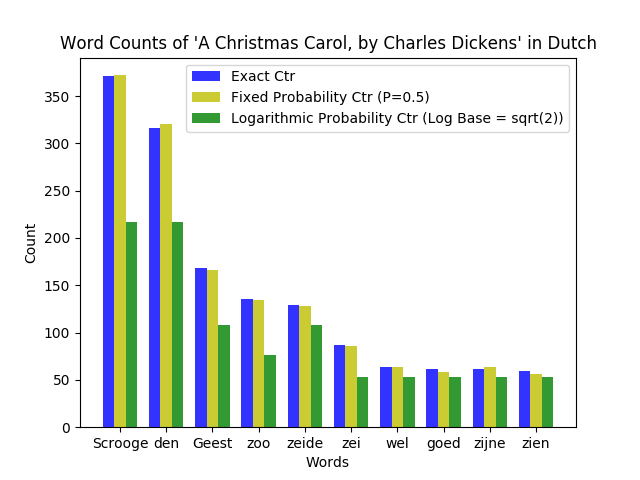
\includegraphics[width=\linewidth]{wordCount_ACC_DU.png}
    \caption{Fig. 1: Counter estimations for the top 10 words.} 
    \label{fig:1}
\end{figure}

It is also possible to understand that the estimated counts of the fixed 
probability counter are far more precise than those of the descending probability
counter.
This is mainly due to the large jumps that occur when estimating the counts of
ACLP. For example, if the counter has the value 13 for the word "Scrooge", its 
estimation will be 217; but if the counter has just one less count, its estimation 
will drop to 153.
This issue would be reduced if the dataset was substantially larger, as the 
"jumps" wouldn't be so large and the deviations would reduce in consequence.
\newline

Finally, I focused on the scatter plots to extract more conclusions.
Figure \ref{fig:2} shows more clearly the problem of ACLP's high deviations.
And what is curious is that in general larger mean average deviations do not 
necessarily mean large deviations in the rank order.

\vspace{-10pt}
\captionsetup[figure]{labelformat=empty}
\begin{figure}[H]
    \centering
    \setlength{\belowcaptionskip}{-12pt}
    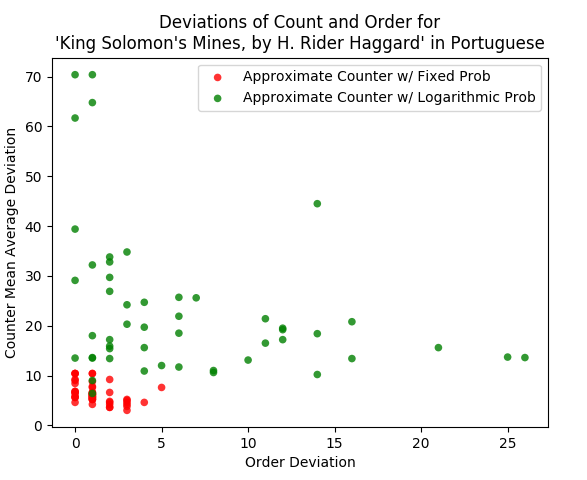
\includegraphics[width=\linewidth]{counterComparison_KSM_PT.png}
    \caption{Fig. 2: Counters deviations for the top 50 words.} 
    \label{fig:2}
\end{figure}

Many of the aspects discussed so far are also possible to understand from the 
results table.
However, I will focus my interpretation of this table on the comparison between 
book translations.

\subsection{Language Comparison}

Let us now closely look at the results table.
This table is actually split into three, one for each counter, for readability
purposes as the original table could not fit in the pages of this document.
Tables 3, 4 and 5 correspond to a portion of the results of the study conducted,
referring to the translations of the book \textit{A Christmas Carol}, by Charles 
Dickens.
There are a few abbreviations to take into account when reading the tables:
ACC (book title); EN, ACFP, ACLP (counters); Lang (language codes); MA Dev, 
MAL Dev, Std Dev, Max Dev (Mean Average, Mean Average Logarithmic, Standard and
Maximum Deviations); MR Err, Avg Err (Mean Relative Error percentage and its averages).
\newline

There seems to be no significant difference in the error percentage between 
translations, and it is supposed to be like so since the algorithms are language 
agnostic.

An interesting discovery also common to all languages is the presence of terms 
like "said" or "replied" in the most frequent words of all chosen books, which 
suggests that these books have a considerable amount of dialogs. 
Also, in most books the names of the main characters always appear on the top 
three words (e.g. "Scrooge" and "Tom" are the first words in all translations of 
\textit{A Christmas Carol} and \textit{The Adventures of Tom Sawyer}), or, if not 
names, their titles (e.g. "sir").

With regards to the top words frequency of each language, there is a tendency 
for Finnish to have smaller counts.
This is generally true for all books, and if we look at the table containing the 
total number of words by book translation (table 2 has a portion of this table 
considering only the book present in the other tables), the reason for this does 
not lie in the fact that the translations to this language require less words; 
rather it suggests that the language has a wider range of vocabulary that spreads 
the counts.

I also dedicated part of my analysis to comparing Dutch and German, as these 
languages are thought to be very similar, so I was interested in knowing if they 
would have similar results as well.
It was a surprise to learn that they had very few similar words on the top 10 rank.
In fact, the ones they had in common were mostly key words related to the context 
of the book, such as "Ghost".
After some research, I understood they differ more than I previously thought, 
as much as Portuguese and Spanish for example.
\newline

The conclusions here presented are the result of speculations based on the few 
books analysed.
In order for them to be more trustworthy, one would have to conduct this study 
with both a larger dataset and additional approaches to the language comparison 
that go beyond the scope of this project.
\newpage

\subsection{Approximate Counters Applicability}

From what we have already seen, there are clear differences between solutions.
The advantages of ACFP were its fidelity to the reality and estimations with very
low error percentages, it presented very good results for the provided dataset.
ACLP on the other hand compensated its lower accuracy with a very economic counting 
strategy.

So what can we take from this?
Well, the study conducted indicates that a fixed probability solution benefits 
the most with medium sized text corpus as the ones tested.
This is mainly due to its high precision where memory costs don't yet weight 
enough to be really considered.
It is my belief that, if the exact word or event counts are not required and 
the intention is to determine only the most common ones, a solution like ACFP is 
very much advisable.

However, if we understand the way these algorithms develop when scaled, there
will be contexts in which a descending probability algorithm will be the best 
alternative.
As the text corpus (or any other type of countable data) scales, the fixed 
probability algorithm remains accurate but starts to cost almost as much as the
exact counting.
In these situations, the logarithmic algorithm actually benefits a lot since, 
as we have discussed, the more frequent are repetitions the smaller 
is the "jump" between estimations of the counters - meaning that the solution 
will have a better accuracy while improving its memory saving as well 
(as the probability of incrementing the counts keeps descending).
This makes the algorithm highly scalable.

%%%%%%%%%%%%%%%%%%%%%%%%%%%%%%%%%%%%%%%%%%%%%%%%%%%%%%%%%%%%%%%%%%%%%%%%%%%%%%%%

\section{Conclusion}

Today's big data companies are concerned with many aspects related to treating 
their information through intelligent algorithms while maintaining reduced 
memory requirements and improving access throughput and transfer speed.
Probabilistic algorithms are very common in such environments and bring great 
value to those who apply them well.
In this report I presented 2 of the most famous probabilistic and approximate 
counters in a word counting context.
They proved to have several advantages and provided a good understanding of the 
potential of solutions around the concepts they are based on.

The study conducted allowed me to learn first hand the probabilistic approach to 
mathematical problems under the discussed context.
It also provided me with the opportunity to learn about language differences in 
a practical and relatively free way, as no restrictions to the literary works 
were provided.

For future work, I believe two alternatives could be considered: implementing 
a floating-point counter solution, another famous probabilistic counter proposed 
by Miklós Csuros; explore sketch algorithms, where there isn't a need to have a 
counter for all unique words.
Both show great potential and would be interesting to be put to test side by side 
with the ones here presented.
\newpage

%%%%%%%%%%%%%%%%%%%%%%%%%%%%%%%%%%%%%%%%%%%%%%%%%%%%%%%%%%%%%%%%%%%%%%%%%%%%%%%%

\bibliography{report.bib} 
\vspace{91pt}

\section*{Appendix}

\begin{table}[H]
\begin{tabular}{@{}cccc@{}}
\toprule
\textbf{Book} & \multicolumn{1}{l|}{\textbf{Lang}} & \textbf{All Words} & \textbf{Relevant Words} \\ \midrule
ACC & \multicolumn{1}{l|}{EN} & 30023     & 14156          \\
    & \multicolumn{1}{l|}{FI} & 23074     & 15671          \\
    & \multicolumn{1}{l|}{GE} & 27182     & 13020          \\
    & \multicolumn{1}{l|}{DU} & 31777     & 15983          \\
    & \multicolumn{1}{l|}{FR} & 35068     & 17637          \\ \bottomrule
\end{tabular}
\caption{Total number of words in all translations of \textit{A Christmas Carol}.}
\end{table}
\newpage

\begin{table}[H]
\centering
\begin{tabular}{@{}cccc@{}}
\toprule
\textbf{Book} & \multicolumn{1}{l|}{\textbf{Lang}} & \textbf{Words} & \textbf{EC} \\ \midrule
ACC  & \multicolumn{1}{l|}{EN}      & Scrooge     & 374       \\
        & \multicolumn{1}{l|}{}     & said        & 221       \\
        & \multicolumn{1}{l|}{}     & upon        & 117       \\
        & \multicolumn{1}{l|}{}     & one         & 100       \\
        & \multicolumn{1}{l|}{}     & Christmas   & 90        \\
        & \multicolumn{1}{l|}{}     & Ghost       & 89        \\
        & \multicolumn{1}{l|}{}     & would       & 85        \\
        & \multicolumn{1}{l|}{}     & Spirit      & 81        \\
        & \multicolumn{1}{l|}{}     & man         & 74        \\
        & \multicolumn{1}{l|}{}     & little      & 66        \\ \cmidrule(l){2-4} 
        & \multicolumn{1}{l|}{FI}   & Scrooge     & 367       \\
        & \multicolumn{1}{l|}{}     & niinkuin    & 100       \\
        & \multicolumn{1}{l|}{}     & henki       & 92        \\
        & \multicolumn{1}{l|}{}     & lausui      & 88        \\
        & \multicolumn{1}{l|}{}     & vastasi     & 79        \\
        & \multicolumn{1}{l|}{}     & kaikki      & 78        \\
        & \multicolumn{1}{l|}{}     & mitään      & 75        \\
        & \multicolumn{1}{l|}{}     & sanoi       & 72        \\
        & \multicolumn{1}{l|}{}     & eikä        & 70        \\
        & \multicolumn{1}{l|}{}     & Bob         & 59        \\ \cmidrule(l){2-4} 
        & \multicolumn{1}{l|}{GE}   & Scrooge     & 311       \\
        & \multicolumn{1}{l|}{}     & sagte       & 219       \\
        & \multicolumn{1}{l|}{}     & Geist       & 159       \\
        & \multicolumn{1}{l|}{}     & hätte       & 61        \\
        & \multicolumn{1}{l|}{}     & rief        & 61        \\
        & \multicolumn{1}{l|}{}     & wurde       & 51        \\
        & \multicolumn{1}{l|}{}     & Scrooges    & 49        \\
        & \multicolumn{1}{l|}{}     & Bob         & 49        \\
        & \multicolumn{1}{l|}{}     & Weihnachten & 48        \\
        & \multicolumn{1}{l|}{}     & sah         & 46        \\ \cmidrule(l){2-4} 
        & \multicolumn{1}{l|}{DU}   & Scrooge     & 371       \\
        & \multicolumn{1}{l|}{}     & den         & 316       \\
        & \multicolumn{1}{l|}{}     & Geest       & 168       \\
        & \multicolumn{1}{l|}{}     & zoo         & 135       \\
        & \multicolumn{1}{l|}{}     & zeide       & 129       \\
        & \multicolumn{1}{l|}{}     & zei         & 87        \\
        & \multicolumn{1}{l|}{}     & wel         & 64        \\
        & \multicolumn{1}{l|}{}     & goed        & 62        \\
        & \multicolumn{1}{l|}{}     & zijne       & 62        \\
        & \multicolumn{1}{l|}{}     & zien        & 59        \\ \cmidrule(l){2-4} 
        & \multicolumn{1}{l|}{FR}   & Scrooge     & 363       \\
        & \multicolumn{1}{l|}{}     & plus        & 209       \\
        & \multicolumn{1}{l|}{}     & dit         & 170       \\
        & \multicolumn{1}{l|}{}     & comme       & 159       \\
        & \multicolumn{1}{l|}{}     & tout        & 149       \\
        & \multicolumn{1}{l|}{}     & bien        & 148       \\
        & \multicolumn{1}{l|}{}     & esprit      & 92        \\
        & \multicolumn{1}{l|}{}     & Noël        & 90        \\
        & \multicolumn{1}{l|}{}     & spectre     & 70        \\
        & \multicolumn{1}{l|}{}     & être        & 69        \\ \bottomrule
\end{tabular}
\caption{Exact counts of the top 10 words in all translations of \textit{A Christmas Carol}.}
\end{table}
\newpage

\begin{table}[H]
\centering
\begin{tabular}{@{}ccccccccc@{}}
\toprule
\textbf{Book} & \multicolumn{1}{l|}{\textbf{Lang}} & \textbf{Words} & \textbf{ACFP} & \textbf{MA Dev} & \textbf{Std Dev} & \textbf{Max Dev} & \textbf{MR Err(\%)} & \textbf{Avg Err(\%)} \\ \midrule
ACC  & \multicolumn{1}{l|}{EN} & Scrooge     & 187          & 9            & 3       & 24      & 2.41              & 7.75         \\
     & \multicolumn{1}{l|}{}   & said        & 108          & 8.2          & 2.88    & 23      & 3.71              &              \\
     & \multicolumn{1}{l|}{}   & upon        & 59           & 7.4          & 3.51    & 13      & 6.32              &              \\
     & \multicolumn{1}{l|}{}   & one         & 52           & 10.8         & 5.02    & 18      & 10.8              &              \\
     & \multicolumn{1}{l|}{}   & Christmas   & 47           & 8            & 2.9     & 22      & 8.89              &              \\
     & \multicolumn{1}{l|}{}   & Ghost       & 47           & 7.4          & 2.88    & 29      & 8.31              &              \\
     & \multicolumn{1}{l|}{}   & would       & 42           & 7            & 2.81    & 13      & 8.24              &              \\
     & \multicolumn{1}{l|}{}   & Spirit      & 39           & 5.2          & 2.3     & 19      & 6.42              &              \\
     & \multicolumn{1}{l|}{}   & man         & 36           & 5.6          & 2.68    & 16      & 7.57              &              \\
     & \multicolumn{1}{l|}{}   & time        & 35           & 7.6          & 4.2     & 16      & 11.52             &              \\ \cmidrule(l){2-9} 
     & \multicolumn{1}{l|}{FI} & Scrooge     & 182          & 14.2         & 6.57    & 39      & 3.87              & 8.85         \\
     & \multicolumn{1}{l|}{}   & niinkuin    & 50           & 8.8          & 3.52    & 18      & 8.8               &              \\
     & \multicolumn{1}{l|}{}   & henki       & 46           & 11.8         & 5.6     & 22      & 12.83             &              \\
     & \multicolumn{1}{l|}{}   & lausui      & 43           & 10.2         & 4.96    & 26      & 11.59             &              \\ 
     & \multicolumn{1}{l|}{}   & kaikki      & 42           & 8.4          & 2.97    & 20      & 10.77             &              \\
     & \multicolumn{1}{l|}{}   & vastasi     & 38           & 5.4          & 2.35    & 13      & 6.84              &              \\
     & \multicolumn{1}{l|}{}   & mitään      & 36           & 6.2          & 2.66    & 11      & 8.27              &              \\
     & \multicolumn{1}{l|}{}   & sanoi       & 34           & 4.4          & 3.29    & 10      & 6.11              &              \\
     & \multicolumn{1}{l|}{}   & eikä        & 33           & 5.8          & 2.49    & 14      & 8.29              &              \\
     & \multicolumn{1}{l|}{}   & Bob         & 29           & 6.6          & 2.74    & 17      & 11.19             &              \\ \cmidrule(l){2-9} 
     & \multicolumn{1}{l|}{GE} & Scrooge     & 154          & 18.4         & 4.83    & 37      & 5.92              & 9.58         \\
     & \multicolumn{1}{l|}{}   & sagte       & 109          & 9.4          & 7.89    & 23      & 4.29              &              \\
     & \multicolumn{1}{l|}{}   & Geist       & 76           & 12           & 3.59    & 27      & 7.55              &              \\
     & \multicolumn{1}{l|}{}   & hätte       & 32           & 7.2          & 3.91    & 17      & 11.8              &              \\
     & \multicolumn{1}{l|}{}   & rief        & 29           & 6.2          & 2.66    & 15      & 10.16             &              \\
     & \multicolumn{1}{l|}{}   & wurde       & 26           & 5.6          & 4.74    & 13      & 10.98             &              \\
     & \multicolumn{1}{l|}{}   & Bob         & 26           & 5.8          & 2.88    & 11      & 11.84             &              \\
     & \multicolumn{1}{l|}{}   & Scrooges    & 25           & 8            & 3.59    & 23      & 16.33             &              \\
     & \multicolumn{1}{l|}{}   & wäre        & 24           & 5            & 4.14    & 11      & 11.11             &              \\
     & \multicolumn{1}{l|}{}   & Weihnachten & 24           & 5.4          & 4.45    & 12      & 11.25             &              \\ \cmidrule(l){2-9} 
     & \multicolumn{1}{l|}{DU} & Scrooge     & 186          & 15.8         & 4.28    & 61      & 4.26              & 6.99         \\
     & \multicolumn{1}{l|}{}   & den         & 160          & 14.4         & 11.4    & 40      & 4.56              &              \\
     & \multicolumn{1}{l|}{}   & Geest       & 83           & 7.2          & 2.97    & 18      & 4.29              &              \\
     & \multicolumn{1}{l|}{}   & zoo         & 67           & 8.8          & 4.11    & 19      & 6.52              &              \\
     & \multicolumn{1}{l|}{}   & zeide       & 64           & 7.6          & 4.95    & 15      & 5.89              &              \\
     & \multicolumn{1}{l|}{}   & zei         & 43           & 6.8          & 5.41    & 15      & 7.82              &              \\
     & \multicolumn{1}{l|}{}   & wel         & 32           & 3.8          & 3.71    & 10      & 5.94              &              \\
     & \multicolumn{1}{l|}{}   & zijne       & 32           & 5.6          & 5.59    & 16      & 9.03              &              \\
     & \multicolumn{1}{l|}{}   & man         & 29           & 4.2          & 6.65    & 20      & 7.5               &              \\
     & \multicolumn{1}{l|}{}   & goed        & 29           & 8.8          & 7.56    & 22      & 14.19             &              \\ \cmidrule(l){2-9} 
     & \multicolumn{1}{l|}{FR} & Scrooge     & 177          & 22           & 4.79    & 55      & 6.06              & 7.08         \\
     & \multicolumn{1}{l|}{}   & plus        & 105          & 8            & 3.24    & 11      & 3.83              &              \\
     & \multicolumn{1}{l|}{}   & dit         & 85           & 5.2          & 6.13    & 18      & 3.06              &              \\
     & \multicolumn{1}{l|}{}   & comme       & 77           & 11.2         & 8.58    & 25      & 7.04              &              \\
     & \multicolumn{1}{l|}{}   & tout        & 76           & 7.4          & 5.47    & 17      & 4.97              &              \\
     & \multicolumn{1}{l|}{}   & bien        & 74           & 11.6         & 6.1     & 24      & 7.84              &              \\
     & \multicolumn{1}{l|}{}   & esprit      & 43           & 7.2          & 2.76    & 28      & 7.83              &              \\
     & \multicolumn{1}{l|}{}   & Noël        & 43           & 9            & 3       & 20      & 10                &              \\
     & \multicolumn{1}{l|}{}   & spectre     & 36           & 7.4          & 3       & 20      & 10.57             &              \\
     & \multicolumn{1}{l|}{}   & être        & 36           & 6.6          & 2.74    & 17      & 9.57              &              \\ \bottomrule
\end{tabular}
\caption{Approximate counts (with fixed probability) of the top 10 words in all translations of \textit{A Christmas Carol}.}
\end{table}
\newpage
\textbf{ }
\newpage

\begin{table}[H]
\centering 
\begin{tabular}{@{}cccccccccc@{}}
\toprule
\textbf{Book} & \multicolumn{1}{l|}{\textbf{Lang}} & \textbf{Words} & \textbf{ACLP} & \textbf{MAL Dev} & \textbf{MA Dev} & \textbf{Std Dev} & \textbf{Max Dev} & \textbf{MR Err(\%)} & \textbf{Avg Err(\%)} \\ \midrule
ACC  & \multicolumn{1}{l|}{EN} & Scrooge     & 13           & 3.1              & 75.1         & 22.6    & 157     & 20.08             & 33.92        \\
     & \multicolumn{1}{l|}{}   & said        & 11           & 3.3              & 83.8         & 46.76   & 168     & 37.92             &              \\
     & \multicolumn{1}{l|}{}   & one         & 10           & 2.3              & 37.5         & 6.75    & 100     & 32.05             &              \\
     & \multicolumn{1}{l|}{}   & upon        & 10           & 2.6              & 46           & 18.08   & 208     & 46                &              \\
     & \multicolumn{1}{l|}{}   & would       & 10           & 3.5              & 38.3         & 8.41    & 63      & 42.56             &              \\
     & \multicolumn{1}{l|}{}   & Spirit      & 10           & 1.9              & 32.3         & 17.4    & 64      & 36.29             &              \\
     & \multicolumn{1}{l|}{}   & Ghost       & 10           & 1.9              & 27.6         & 8.97    & 68      & 32.47             &              \\
     & \multicolumn{1}{l|}{}   & Christmas   & 9            & 1.9              & 24.5         & 14.77   & 44      & 30.25             &              \\
     & \multicolumn{1}{l|}{}   & could       & 9            & 2.6              & 18.2         & 4.31    & 37      & 24.59             &              \\
     & \multicolumn{1}{l|}{}   & man         & 9            & 3.1              & 22.8         & 6.3     & 42      & 34.55             &              \\ \cmidrule(l){2-10} 
     & \multicolumn{1}{l|}{FI} & Scrooge     & 13           & 3.4              & 92.7         & 68.35   & 214     & 25.26             & 34.69        \\
     & \multicolumn{1}{l|}{}   & henki       & 10           & 2.8              & 22.9         & 5.41    & 47      & 22.9              &              \\
     & \multicolumn{1}{l|}{}   & niinkuin    & 10           & 2.7              & 38           & 13.79   & 61      & 41.3              &              \\
     & \multicolumn{1}{l|}{}   & eikä        & 9            & 2.1              & 34.5         & 8.63    & 65      & 39.2              &              \\
     & \multicolumn{1}{l|}{}   & vastasi     & 9            & 2.1              & 24           & 10.68   & 41      & 30.77             &              \\
     & \multicolumn{1}{l|}{}   & kaikki      & 9            & 2.4              & 36.4         & 10.2    & 138     & 46.08             &              \\
     & \multicolumn{1}{l|}{}   & lausui      & 9            & 3.3              & 29.6         & 8.83    & 49      & 39.47             &              \\
     & \multicolumn{1}{l|}{}   & sanoi       & 9            & 3                & 23.6         & 5.02    & 46      & 32.78             &              \\
     & \multicolumn{1}{l|}{}   & Cratchit    & 9            & 2.6              & 17.4         & 6.8     & 44      & 24.86             &              \\
     & \multicolumn{1}{l|}{}   & koko        & 8            & 2.3              & 26.1         & 8.63    & 94      & 44.24             &              \\ \cmidrule(l){2-10} 
     & \multicolumn{1}{l|}{GE} & Scrooge     & 13           & 3                & 83.2         & 31.09   & 158     & 26.75             & 31.27        \\
     & \multicolumn{1}{l|}{}   & sagte       & 12           & 3                & 73.5         & 36.13   & 111     & 33.56             &              \\
     & \multicolumn{1}{l|}{}   & Geist       & 11           & 2.1              & 51.9         & 19.71   & 149     & 32.64             &              \\
     & \multicolumn{1}{l|}{}   & hätte       & 9            & 1.7              & 14.9         & 8.51    & 47      & 24.43             &              \\
     & \multicolumn{1}{l|}{}   & rief        & 9            & 1.7              & 14.7         & 4.59    & 24      & 24.1              &              \\
     & \multicolumn{1}{l|}{}   & Scrooges    & 8            & 3.1              & 18.3         & 8.99    & 25      & 35.88             &              \\
     & \multicolumn{1}{l|}{}   & sei         & 8            & 2.1              & 18.4         & 9.56    & 59      & 37.55             &              \\
     & \multicolumn{1}{l|}{}   & wäre        & 8            & 2.6              & 15.9         & 5.5     & 27      & 32.45             &              \\
     & \multicolumn{1}{l|}{}   & mehr        & 8            & 2.3              & 10.3         & 4.09    & 31      & 22.89             &              \\
     & \multicolumn{1}{l|}{}   & Weihnachten & 8            & 2.3              & 13.1         & 7.84    & 28      & 27.29             &              \\ \cmidrule(l){2-10} 
     & \multicolumn{1}{l|}{DU} & den         & 13           & 3.6              & 107.6        & 22.46   & 263     & 29                & 32.78        \\
     & \multicolumn{1}{l|}{}   & Scrooge     & 13           & 2.9              & 79.1         & 9.25    & 163     & 25.03             &              \\
     & \multicolumn{1}{l|}{}   & zeide       & 11           & 2.7              & 42.6         & 8.07    & 92      & 25.36             &              \\
     & \multicolumn{1}{l|}{}   & Geest       & 11           & 3.3              & 38.9         & 10.57   & 109     & 28.81             &              \\
     & \multicolumn{1}{l|}{}   & zoo         & 10           & 2.5              & 38.2         & 17.86   & 88      & 29.61             &              \\
     & \multicolumn{1}{l|}{}   & wel         & 9            & 2.7              & 29           & 6.41    & 50      & 33.33             &              \\
     & \multicolumn{1}{l|}{}   & goed        & 9            & 2.7              & 28.2         & 6.35    & 89      & 44.06             &              \\
     & \multicolumn{1}{l|}{}   & zijne       & 9            & 1.9              & 22.8         & 6.51    & 46      & 36.77             &              \\
     & \multicolumn{1}{l|}{}   & zei         & 9            & 2.4              & 29.9         & 13.2    & 52      & 53.39             &              \\
     & \multicolumn{1}{l|}{}   & zien        & 9            & 1.7              & 26.5         & 6.79    & 46      & 42.74             &              \\ \cmidrule(l){2-10} 
     & \multicolumn{1}{l|}{FR} & Scrooge     & 13           & 3.5              & 95.1         & 47.19   & 210     & 26.2              & 31.02        \\
     & \multicolumn{1}{l|}{}   & plus        & 12           & 3                & 53.8         & 32.77   & 133     & 25.74             &              \\
     & \multicolumn{1}{l|}{}   & comme       & 11           & 2.1              & 68.6         & 9.87    & 138     & 40.35             &              \\
     & \multicolumn{1}{l|}{}   & bien        & 11           & 2.9              & 42.6         & 6.8     & 83      & 26.79             &              \\
     & \multicolumn{1}{l|}{}   & tout        & 11           & 2.7              & 49.1         & 24.12   & 73      & 32.95             &              \\
     & \multicolumn{1}{l|}{}   & dit         & 11           & 2.2              & 54           & 14.63   & 160     & 36.49             &              \\
     & \multicolumn{1}{l|}{}   & esprit      & 10           & 2.9              & 29           & 18.21   & 61      & 31.52             &              \\
     & \multicolumn{1}{l|}{}   & spectre     & 9            & 3.5              & 35.1         & 13.11   & 64      & 39                &              \\
     & \multicolumn{1}{l|}{}   & aussi       & 9            & 2.5              & 16.3         & 12.68   & 38      & 23.29             &              \\
     & \multicolumn{1}{l|}{}   & être        & 9            & 2.3              & 19.2         & 6.69    & 84      & 27.83             &              \\ \bottomrule
\end{tabular}
\caption{Approximate counts (with descending probability) of the top 10 words in all translations of \textit{A Christmas Carol}.}
\end{table}

\end{document}
